%%%%%%%%%%%%%%%%%%%%%%%%%%%%%%%%%%%%%%%%%
%  My documentation report
%  Objetive: Explain what I did and how, so someone can continue with the investigation
%
% Important note:
% Chapter heading images should have a 2:1 width:height ratio,
% e.g. 920px width and 460px height.
%
%%%%%%%%%%%%%%%%%%%%%%%%%%%%%%%%%%%%%%%%%

%----------------------------------------------------------------------------------------
%	PACKAGES AND OTHER DOCUMENT CONFIGURATIONS
%----------------------------------------------------------------------------------------

\documentclass[11pt,fleqn]{book} % Default font size and left-justified equations

\usepackage[top=3cm,bottom=3cm,left=3.2cm,right=3.2cm,headsep=10pt,letterpaper]{geometry} % Page margins

\usepackage{xcolor} % Required for specifying colors by name
\definecolor{ocre}{RGB}{52,177,201} % Define the orange color used for highlighting throughout the book

% Font Settings
\usepackage{avant} % Use the Avantgarde font for headings
%\usepackage{times} % Use the Times font for headings
\usepackage{mathptmx} % Use the Adobe Times Roman as the default text font together with math symbols from the Sym­bol, Chancery and Com­puter Modern fonts

\usepackage{microtype} % Slightly tweak font spacing for aesthetics
\usepackage[utf8]{inputenc} % Required for including letters with accents
\usepackage[T1]{fontenc} % Use 8-bit encoding that has 256 glyphs

%Tables
\usepackage{tabularx}
\usepackage{longtable,tabu}

% Bibliography
\usepackage[style=alphabetic,sorting=nyt,sortcites=true,autopunct=true,babel=hyphen,hyperref=true,abbreviate=false,backref=true,backend=biber]{biblatex}
\addbibresource{bibliography.bib} % BibTeX bibliography file
\defbibheading{bibempty}{}

\input{structure} % Insert the commands.tex file which contains the majority of the structure behind the template

\begin{document}

%----------------------------------------------------------------------------------------
%	TITLE PAGE
%----------------------------------------------------------------------------------------

\begingroup
\thispagestyle{empty}
\AddToShipoutPicture*{\put(0,0){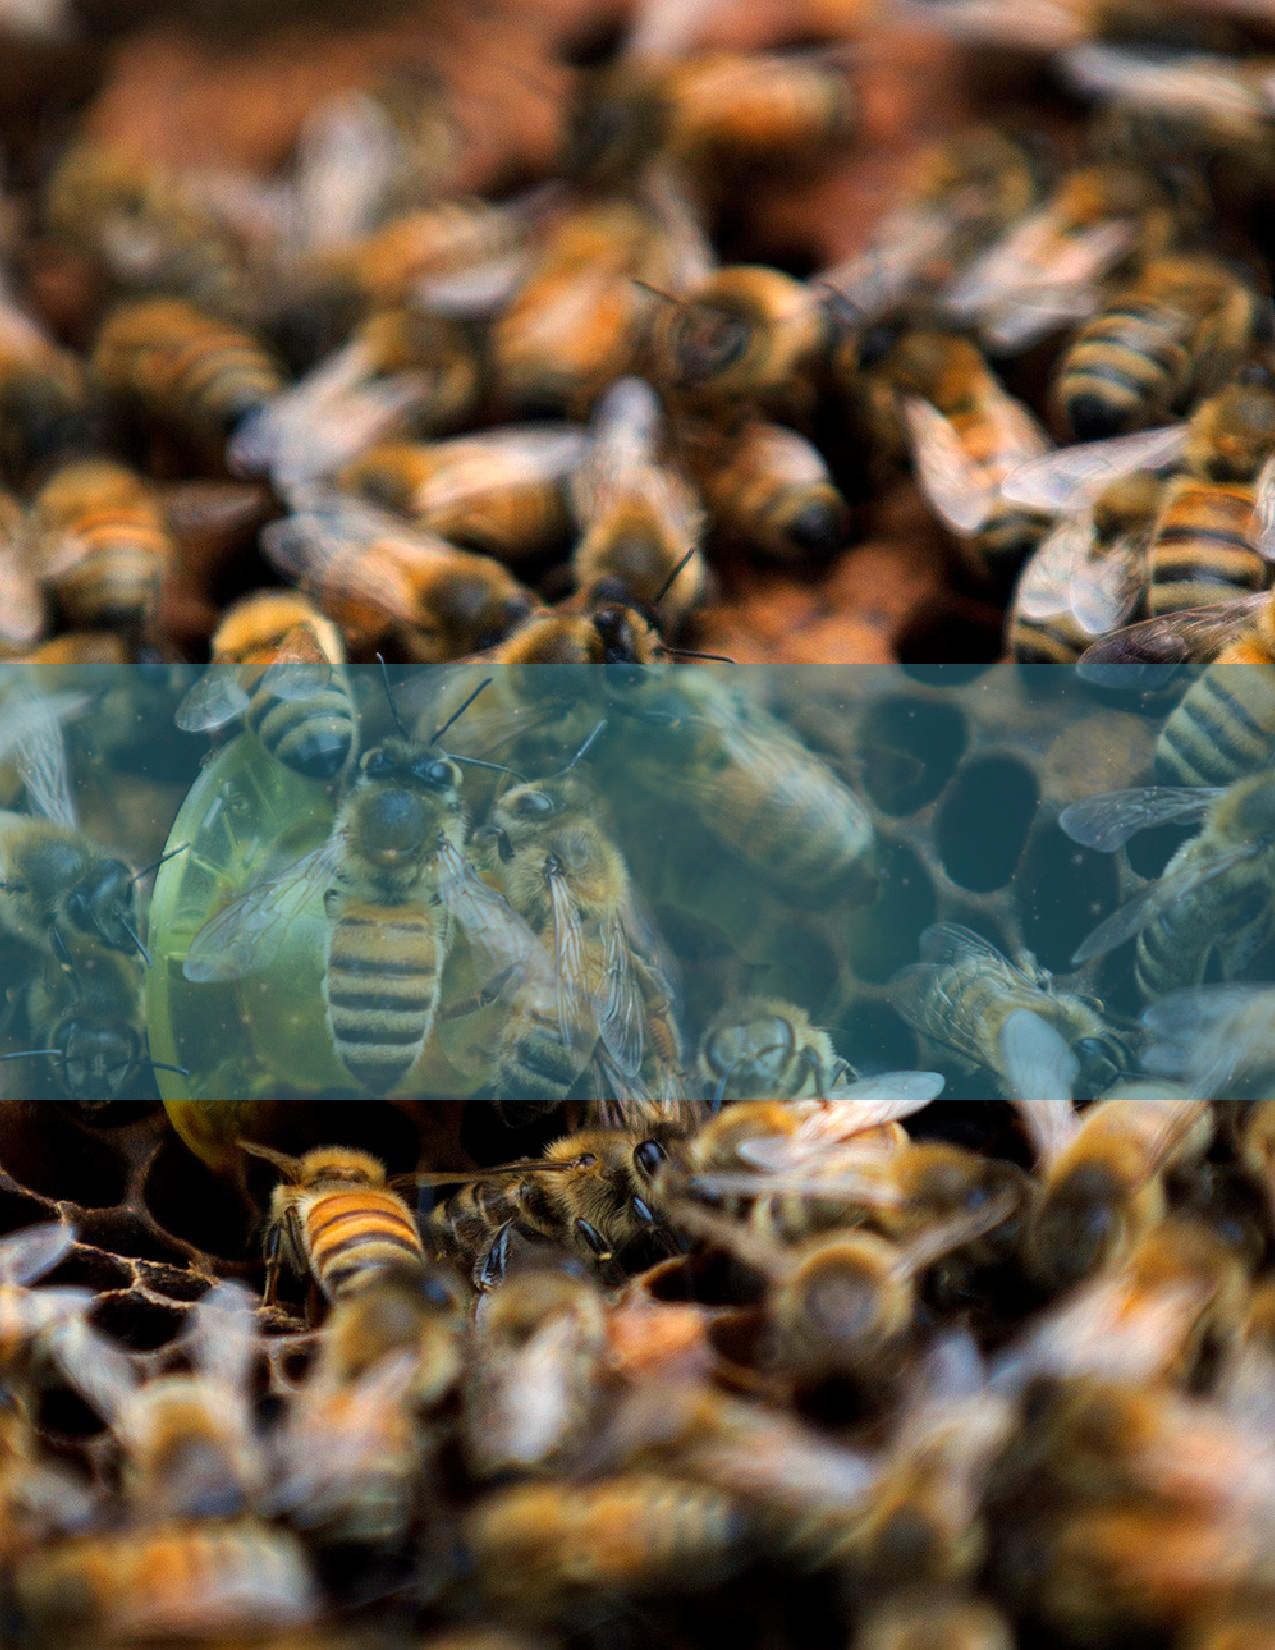
\includegraphics[scale=1.25]{cover.png}}} % Image background
\centering
\vspace*{4cm}
\par\normalfont\fontsize{35}{35}\sffamily\selectfont
\textbf{\color{white}Data Mining for Bee Micro-sensors}\\
{\Huge\color{white} Laboratorio Nacional de Análisis y Síntesis Ecológica}\par % Book title
\vspace*{0.2cm}
%Add all the collaborators
%{\LARGE\color{white} Laboratorio Nacional de Análisis y Síntesis Ecológica}\par % Author name
{\LARGE\color{white} Framework Developed by:\\ Ulises Olivares, Gloria Ruiz, Maria J. Aguilar, Oliverio Delgado, Francisco J. Balvino, Mauricio Quesada }\par % Author name
\endgroup

%----------------------------------------------------------------------------------------
%	COPYRIGHT PAGE
%----------------------------------------------------------------------------------------

\newpage
~\vfill
\thispagestyle{empty}

%\noindent Copyright \copyright\ 2014 Andrea Hidalgo\\ % Copyright notice

\noindent \textsc{High Performance Computing applied to biological sciences, Universidad Nacional Autónoma de México - Escuela Nacional de de Estudios Superiores Unidad Morelia - Laboratorio Nacional de Análisis y Síntesis Ecológica }\\

\noindent  This work was supported by grants from Consejo Nacional de Ciencia y Tecnología (CONACyT: Laboratorio Nacional de Análisis y Síntesis Ecológica U-3-2015-2-250996, CONACYT and CONACyT: Propuesta para eldesarrollo de una infraestructura tecnológica para lacreación de repositorios masivos de datos biológicos con fines de conservación y análisis de información I0028-2015-02-271432, CONACYT).\\ % License information

\noindent \textit{First release, April 2017} % Printing/edition date

%----------------------------------------------------------------------------------------
%	TABLE OF CONTENTS
%----------------------------------------------------------------------------------------

\chapterimage{head1.jpg} % Table of contents heading image

\pagestyle{empty} % No headers

\tableofcontents % Print the table of contents itself

%\cleardoublepage % Forces the first chapter to start on an odd page so it's on the right

\pagestyle{fancy} % Print headers again

%INSERT_CONTENT_HERE
\part{Morelia Hive 1}
\chapterimage{head2.jpg} % Chapter heading image 
\chapter{Introduction} 
\normalsize%
\section*{Introduction}%
The main propose of this document  is to show a concise report about the activity of bees and behavior in a specific period of time. This report also shows a complete analysis of the most active hours.\newline%
\newline%
Tis report corresponds to a period of time of 123 day(s). From 2016{-}07{-}02 to 2016{-}12{-}02. During this period of time, a total amount of 18653 lectures were registered from 156 different bees. There exist a total of 26 non{-}active days. We define an 'active day' if there is more than one observation. (see Figure1.1).\newline%
\newline%
%


\begin{figure}[h!]%
\centering%
\includegraphics[width=315px]{chartNumLectures.png}%
\caption{Days with and without Empty Reads}%
\end{figure}

\chapterimage{head3.jpg} % Chapter heading image 
\chapter{Analysis of Raw Data} 
\normalsize%
\subsection*{Activity Per Day of Raw Data}%
This section addresses the analysis of raw data. Which implies that this date is presented without filters or a data preprocessing step to clean the data. This section presents severalgraphs which reflects the behavior of a beehive during a specific period of time.%


\begin{figure}[h!]%
\centering%
\includegraphics[width=400px]{observationsPerdayUnclean.png}%
\caption{Number of Observations per Day}%
\end{figure}

%
\begin{longtabu}{| c | c | c | c |}%
\hline%
Day&Date&\# Observations&\# Bees per day\\%
\hline%
1&2016{-}07{-}02&1&1\\%
\hline%
2&2016{-}07{-}03&1&1\\%
\hline%
3&2016{-}07{-}08&50&8\\%
\hline%
4&2016{-}07{-}09&145&11\\%
\hline%
5&2016{-}07{-}10&115&10\\%
\hline%
6&2016{-}07{-}11&50&7\\%
\hline%
7&2016{-}07{-}12&21&5\\%
\hline%
8&2016{-}07{-}13&26&7\\%
\hline%
9&2016{-}07{-}14&65&4\\%
\hline%
10&2016{-}07{-}15&731&14\\%
\hline%
11&2016{-}07{-}16&510&11\\%
\hline%
12&2016{-}07{-}17&68&5\\%
\hline%
13&2016{-}07{-}18&43&3\\%
\hline%
14&2016{-}07{-}19&32&3\\%
\hline%
15&2016{-}07{-}20&33&3\\%
\hline%
16&2016{-}07{-}21&16&3\\%
\hline%
17&2016{-}07{-}22&6&2\\%
\hline%
18&2016{-}07{-}23&342&16\\%
\hline%
19&2016{-}07{-}24&256&12\\%
\hline%
20&2016{-}07{-}25&66&8\\%
\hline%
21&2016{-}07{-}26&105&7\\%
\hline%
22&2016{-}07{-}27&29&5\\%
\hline%
23&2016{-}07{-}28&21&5\\%
\hline%
24&2016{-}07{-}29&37&6\\%
\hline%
25&2016{-}07{-}30&27&4\\%
\hline%
26&2016{-}07{-}31&26&4\\%
\hline%
27&2016{-}08{-}01&41&5\\%
\hline%
28&2016{-}08{-}02&39&5\\%
\hline%
29&2016{-}08{-}03&35&5\\%
\hline%
30&2016{-}08{-}04&21&5\\%
\hline%
31&2016{-}08{-}05&98&5\\%
\hline%
32&2016{-}08{-}06&15&6\\%
\hline%
33&2016{-}08{-}07&175&15\\%
\hline%
34&2016{-}08{-}08&147&13\\%
\hline%
35&2016{-}08{-}09&131&11\\%
\hline%
36&2016{-}08{-}10&82&8\\%
\hline%
37&2016{-}08{-}11&85&7\\%
\hline%
38&2016{-}08{-}12&239&9\\%
\hline%
39&2016{-}08{-}13&53&8\\%
\hline%
40&2016{-}08{-}14&113&7\\%
\hline%
41&2016{-}08{-}15&269&12\\%
\hline%
42&2016{-}08{-}16&271&14\\%
\hline%
43&2016{-}08{-}17&98&7\\%
\hline%
44&2016{-}08{-}18&378&12\\%
\hline%
45&2016{-}08{-}19&219&8\\%
\hline%
46&2016{-}08{-}20&356&8\\%
\hline%
47&2016{-}08{-}21&83&7\\%
\hline%
48&2016{-}08{-}22&49&7\\%
\hline%
49&2016{-}08{-}23&48&4\\%
\hline%
50&2016{-}08{-}24&52&5\\%
\hline%
51&2016{-}08{-}25&27&4\\%
\hline%
52&2016{-}08{-}26&84&6\\%
\hline%
53&2016{-}09{-}20&77&3\\%
\hline%
54&2016{-}09{-}21&68&2\\%
\hline%
55&2016{-}09{-}22&104&3\\%
\hline%
56&2016{-}09{-}23&21&2\\%
\hline%
57&2016{-}09{-}24&5&1\\%
\hline%
58&2016{-}09{-}25&4&1\\%
\hline%
59&2016{-}09{-}26&10&1\\%
\hline%
60&2016{-}09{-}27&6&1\\%
\hline%
61&2016{-}09{-}28&4&1\\%
\hline%
62&2016{-}09{-}29&7&1\\%
\hline%
63&2016{-}09{-}30&7&1\\%
\hline%
64&2016{-}10{-}01&9&1\\%
\hline%
65&2016{-}10{-}02&10&1\\%
\hline%
66&2016{-}10{-}03&3&1\\%
\hline%
67&2016{-}10{-}04&3&2\\%
\hline%
68&2016{-}10{-}07&3&1\\%
\hline%
69&2016{-}10{-}09&2271&14\\%
\hline%
70&2016{-}10{-}10&19&7\\%
\hline%
71&2016{-}10{-}11&2&2\\%
\hline%
72&2016{-}10{-}12&237&7\\%
\hline%
73&2016{-}10{-}13&21&3\\%
\hline%
74&2016{-}10{-}14&28&4\\%
\hline%
75&2016{-}10{-}15&22&6\\%
\hline%
76&2016{-}10{-}16&569&3\\%
\hline%
77&2016{-}10{-}17&234&7\\%
\hline%
78&2016{-}10{-}18&40&6\\%
\hline%
79&2016{-}10{-}19&44&5\\%
\hline%
80&2016{-}10{-}20&39&3\\%
\hline%
81&2016{-}10{-}21&47&5\\%
\hline%
82&2016{-}10{-}22&38&4\\%
\hline%
83&2016{-}10{-}23&66&4\\%
\hline%
84&2016{-}10{-}24&169&3\\%
\hline%
85&2016{-}10{-}25&116&3\\%
\hline%
86&2016{-}10{-}26&52&3\\%
\hline%
87&2016{-}10{-}27&298&5\\%
\hline%
88&2016{-}10{-}28&87&7\\%
\hline%
89&2016{-}10{-}29&59&5\\%
\hline%
90&2016{-}10{-}30&41&6\\%
\hline%
91&2016{-}10{-}31&46&5\\%
\hline%
92&2016{-}11{-}01&95&6\\%
\hline%
93&2016{-}11{-}02&114&7\\%
\hline%
94&2016{-}11{-}03&36&7\\%
\hline%
95&2016{-}11{-}04&26&5\\%
\hline%
96&2016{-}11{-}05&11&4\\%
\hline%
97&2016{-}11{-}06&19&6\\%
\hline%
98&2016{-}11{-}07&123&6\\%
\hline%
99&2016{-}11{-}08&359&14\\%
\hline%
100&2016{-}11{-}09&134&8\\%
\hline%
101&2016{-}11{-}10&2110&6\\%
\hline%
102&2016{-}11{-}11&97&7\\%
\hline%
103&2016{-}11{-}12&282&7\\%
\hline%
104&2016{-}11{-}13&309&5\\%
\hline%
105&2016{-}11{-}14&78&7\\%
\hline%
106&2016{-}11{-}15&103&6\\%
\hline%
107&2016{-}11{-}16&51&6\\%
\hline%
108&2016{-}11{-}17&1357&5\\%
\hline%
109&2016{-}11{-}18&148&6\\%
\hline%
110&2016{-}11{-}19&592&5\\%
\hline%
111&2016{-}11{-}20&58&6\\%
\hline%
112&2016{-}11{-}21&63&5\\%
\hline%
113&2016{-}11{-}22&46&6\\%
\hline%
114&2016{-}11{-}23&39&5\\%
\hline%
115&2016{-}11{-}24&46&5\\%
\hline%
116&2016{-}11{-}25&40&5\\%
\hline%
117&2016{-}11{-}26&26&5\\%
\hline%
118&2016{-}11{-}27&31&3\\%
\hline%
119&2016{-}11{-}28&392&3\\%
\hline%
120&2016{-}11{-}29&80&4\\%
\hline%
121&2016{-}11{-}30&179&4\\%
\hline%
122&2016{-}12{-}01&16&3\\%
\hline%
123&2016{-}12{-}02&677&2\\%
\hline%
\hline%
{-}{-}&Average&151&5\\%
\hline%
\hline%
\end{longtabu}

%
\subsection*{Bee Life Cycle}%
In this section is analyzed the Life Cycle of each bee in the hive%
\begin{longtabu}{| c | c | c |}%
\hline%
\hline%
Register&Bee ID&Life Cycle in Days\\%
\hline%
\hline%
1&0004&1\\%
\hline%
2&0005&1\\%
\hline%
3&0006&1\\%
\hline%
4&0016&1\\%
\hline%
5&0023&1\\%
\hline%
6&0024&5\\%
\hline%
7&0027&1\\%
\hline%
8&0029&8\\%
\hline%
9&0031&1\\%
\hline%
10&0053&5\\%
\hline%
11&0055&1\\%
\hline%
12&0056&1\\%
\hline%
13&0060&1\\%
\hline%
14&0061&1\\%
\hline%
15&0062&1\\%
\hline%
16&0063&6\\%
\hline%
17&0064&1\\%
\hline%
18&0068&16\\%
\hline%
19&0071&1\\%
\hline%
20&0075&5\\%
\hline%
21&0077&18\\%
\hline%
22&0079&122\\%
\hline%
23&0081&1\\%
\hline%
24&0082&1\\%
\hline%
25&0083&1\\%
\hline%
26&0087&2\\%
\hline%
27&0090&3\\%
\hline%
28&0093&1\\%
\hline%
29&0094&1\\%
\hline%
30&0095&1\\%
\hline%
31&0096&1\\%
\hline%
32&0103&1\\%
\hline%
33&0108&17\\%
\hline%
34&0112&1\\%
\hline%
35&0118&1\\%
\hline%
36&0130&23\\%
\hline%
37&0137&5\\%
\hline%
38&0145&3\\%
\hline%
39&0146&2\\%
\hline%
40&0153&3\\%
\hline%
41&0154&1\\%
\hline%
42&0155&1\\%
\hline%
43&0156&2\\%
\hline%
44&0157&2\\%
\hline%
45&0158&1\\%
\hline%
46&0162&3\\%
\hline%
47&0165&2\\%
\hline%
48&0174&1\\%
\hline%
49&0188&7\\%
\hline%
50&0189&2\\%
\hline%
51&0194&1\\%
\hline%
52&0203&1\\%
\hline%
53&0207&1\\%
\hline%
54&0208&2\\%
\hline%
55&0212&16\\%
\hline%
56&0213&27\\%
\hline%
57&0215&1\\%
\hline%
58&0218&1\\%
\hline%
59&0220&1\\%
\hline%
60&0223&117\\%
\hline%
61&0234&18\\%
\hline%
62&0235&2\\%
\hline%
63&0237&1\\%
\hline%
64&0250&1\\%
\hline%
65&0256&20\\%
\hline%
66&0257&3\\%
\hline%
67&0258&1\\%
\hline%
68&0261&1\\%
\hline%
69&0264&14\\%
\hline%
70&0266&20\\%
\hline%
71&0267&20\\%
\hline%
72&0270&1\\%
\hline%
73&0273&3\\%
\hline%
74&0276&9\\%
\hline%
75&0278&1\\%
\hline%
76&0282&1\\%
\hline%
77&0283&6\\%
\hline%
78&0286&1\\%
\hline%
79&0287&1\\%
\hline%
80&0290&14\\%
\hline%
81&0292&4\\%
\hline%
82&0295&1\\%
\hline%
83&0296&1\\%
\hline%
84&0304&1\\%
\hline%
85&0307&3\\%
\hline%
86&0309&1\\%
\hline%
87&0311&5\\%
\hline%
88&0312&1\\%
\hline%
89&0314&1\\%
\hline%
90&0315&1\\%
\hline%
91&0316&3\\%
\hline%
92&0318&1\\%
\hline%
93&0319&1\\%
\hline%
94&0321&1\\%
\hline%
95&0324&1\\%
\hline%
96&0327&1\\%
\hline%
97&0330&6\\%
\hline%
98&0331&1\\%
\hline%
99&0332&1\\%
\hline%
100&0333&1\\%
\hline%
101&0336&1\\%
\hline%
102&0340&1\\%
\hline%
103&0341&11\\%
\hline%
104&0342&7\\%
\hline%
105&0354&1\\%
\hline%
106&0383&1\\%
\hline%
107&0391&1\\%
\hline%
108&0431&1\\%
\hline%
109&0483&1\\%
\hline%
110&0484&4\\%
\hline%
111&0488&1\\%
\hline%
112&0498&1\\%
\hline%
113&0528&1\\%
\hline%
114&0544&15\\%
\hline%
115&0546&1\\%
\hline%
116&0551&1\\%
\hline%
117&0553&27\\%
\hline%
118&0568&1\\%
\hline%
119&0569&1\\%
\hline%
120&0595&1\\%
\hline%
121&0598&1\\%
\hline%
122&0604&1\\%
\hline%
123&0605&1\\%
\hline%
124&0608&4\\%
\hline%
125&0610&27\\%
\hline%
126&0612&2\\%
\hline%
127&0616&9\\%
\hline%
128&0626&1\\%
\hline%
129&0627&1\\%
\hline%
130&0634&1\\%
\hline%
131&0636&22\\%
\hline%
132&0642&2\\%
\hline%
133&0643&13\\%
\hline%
134&0652&34\\%
\hline%
135&0668&1\\%
\hline%
136&0672&1\\%
\hline%
137&0674&1\\%
\hline%
138&0675&10\\%
\hline%
139&0676&18\\%
\hline%
140&0678&15\\%
\hline%
141&0683&2\\%
\hline%
142&0694&1\\%
\hline%
143&0697&1\\%
\hline%
144&0701&1\\%
\hline%
145&0711&1\\%
\hline%
146&0717&25\\%
\hline%
147&0724&24\\%
\hline%
148&0735&18\\%
\hline%
149&0738&18\\%
\hline%
150&0744&1\\%
\hline%
151&0746&2\\%
\hline%
152&0747&3\\%
\hline%
153&0754&1\\%
\hline%
154&0777&1\\%
\hline%
155&0795&1\\%
\hline%
156&0137&1\\%
\hline%
\hline%
{-}{-}&Average&6\\%
\hline%
\hline%
\end{longtabu}%


\begin{figure}[h!]%
\centering%
\includegraphics[width=400px]{differentBeesPerdayUnclean.png}%
\caption{Different Bees Per Day}%
\end{figure}

%


\begin{figure}[h!]%
\centering%
\includegraphics[width=400px]{beeLifeCycleUnclean.png}%
\caption{Bee Life cycle in days}%
\end{figure}

%


\begin{figure}[h!]%
\centering%
\includegraphics[width=400px]{pieBeeLifeCycleUnclean.png}%
\caption{Bee Life cycle in days}%
\end{figure}

%
\subsection*{Analysis of Activity per Hour}%


\begin{figure}[h!]%
\centering%
\includegraphics[width=400px]{histogramUnclean.png}%
\caption{Histogram of frequencies per hour}%
\end{figure}

%


\begin{figure}[h!]%
\centering%
\includegraphics[width=400px]{histogramStdUnclean.png}%
\caption{Histogram of frequencies per hour. It includes standard deviation}%
\end{figure}

\chapterimage{head4.jpg} % Chapter heading image 
\chapter{Analysis of Clean Data}
\normalsize%
\subsection*{Activity Per Day of Clean Data}%
In this section is presented an analysis of input data. During this analysis some filters were applied. One of these filters is the definition of a threshold which removes all the observations that fall in a period of time less than 60 seconds. This preprocessing step tends to  remove all the lost chips which generated unnecessary and repeated registers %


\begin{figure}[h!]%
\centering%
\includegraphics[width=400px]{observationsPerdayClean.png}%
\caption{Number of Observations per Day}%
\end{figure}

%
\begin{longtabu}{| c | c | c | c |}%
\hline%
Day&Date&\# Observations&\# Bees per day\\%
\hline%
1&2016{-}07{-}08&9&3\\%
\hline%
2&2016{-}07{-}09&35&10\\%
\hline%
3&2016{-}07{-}10&42&8\\%
\hline%
4&2016{-}07{-}11&33&5\\%
\hline%
5&2016{-}07{-}12&12&4\\%
\hline%
6&2016{-}07{-}13&16&5\\%
\hline%
7&2016{-}07{-}14&16&3\\%
\hline%
8&2016{-}07{-}15&143&8\\%
\hline%
9&2016{-}07{-}16&69&7\\%
\hline%
10&2016{-}07{-}17&31&5\\%
\hline%
11&2016{-}07{-}18&20&3\\%
\hline%
12&2016{-}07{-}19&22&3\\%
\hline%
13&2016{-}07{-}20&26&3\\%
\hline%
14&2016{-}07{-}21&12&2\\%
\hline%
15&2016{-}07{-}22&4&2\\%
\hline%
16&2016{-}07{-}23&86&10\\%
\hline%
17&2016{-}07{-}24&60&11\\%
\hline%
18&2016{-}07{-}25&24&4\\%
\hline%
19&2016{-}07{-}26&36&7\\%
\hline%
20&2016{-}07{-}27&19&4\\%
\hline%
21&2016{-}07{-}28&13&3\\%
\hline%
22&2016{-}07{-}29&25&4\\%
\hline%
23&2016{-}07{-}30&19&4\\%
\hline%
24&2016{-}07{-}31&20&4\\%
\hline%
25&2016{-}08{-}01&28&5\\%
\hline%
26&2016{-}08{-}02&25&5\\%
\hline%
27&2016{-}08{-}03&22&5\\%
\hline%
28&2016{-}08{-}04&15&4\\%
\hline%
29&2016{-}08{-}05&23&5\\%
\hline%
30&2016{-}08{-}06&5&1\\%
\hline%
31&2016{-}08{-}07&52&10\\%
\hline%
32&2016{-}08{-}08&74&8\\%
\hline%
33&2016{-}08{-}09&65&11\\%
\hline%
34&2016{-}08{-}10&43&8\\%
\hline%
35&2016{-}08{-}11&39&7\\%
\hline%
36&2016{-}08{-}12&41&8\\%
\hline%
37&2016{-}08{-}13&40&7\\%
\hline%
38&2016{-}08{-}14&43&6\\%
\hline%
39&2016{-}08{-}15&40&5\\%
\hline%
40&2016{-}08{-}16&47&9\\%
\hline%
41&2016{-}08{-}17&52&7\\%
\hline%
42&2016{-}08{-}18&63&8\\%
\hline%
43&2016{-}08{-}19&62&7\\%
\hline%
44&2016{-}08{-}20&64&7\\%
\hline%
45&2016{-}08{-}21&37&6\\%
\hline%
46&2016{-}08{-}22&32&5\\%
\hline%
47&2016{-}08{-}23&35&4\\%
\hline%
48&2016{-}08{-}24&35&4\\%
\hline%
49&2016{-}08{-}25&20&4\\%
\hline%
50&2016{-}08{-}26&14&4\\%
\hline%
51&2016{-}09{-}20&9&1\\%
\hline%
52&2016{-}09{-}21&4&1\\%
\hline%
53&2016{-}09{-}22&10&2\\%
\hline%
54&2016{-}09{-}23&5&2\\%
\hline%
55&2016{-}09{-}25&2&1\\%
\hline%
56&2016{-}09{-}26&2&1\\%
\hline%
57&2016{-}09{-}27&2&1\\%
\hline%
58&2016{-}09{-}28&3&1\\%
\hline%
59&2016{-}09{-}29&3&1\\%
\hline%
60&2016{-}09{-}30&4&1\\%
\hline%
61&2016{-}10{-}01&4&1\\%
\hline%
62&2016{-}10{-}02&4&1\\%
\hline%
63&2016{-}10{-}03&2&1\\%
\hline%
64&2016{-}10{-}04&1&1\\%
\hline%
65&2016{-}10{-}09&8&3\\%
\hline%
66&2016{-}10{-}10&2&2\\%
\hline%
67&2016{-}10{-}12&8&5\\%
\hline%
68&2016{-}10{-}13&5&2\\%
\hline%
69&2016{-}10{-}14&8&3\\%
\hline%
70&2016{-}10{-}15&12&4\\%
\hline%
71&2016{-}10{-}16&21&3\\%
\hline%
72&2016{-}10{-}17&27&4\\%
\hline%
73&2016{-}10{-}18&19&3\\%
\hline%
74&2016{-}10{-}19&29&3\\%
\hline%
75&2016{-}10{-}20&26&3\\%
\hline%
76&2016{-}10{-}21&32&4\\%
\hline%
77&2016{-}10{-}22&25&3\\%
\hline%
78&2016{-}10{-}23&37&3\\%
\hline%
79&2016{-}10{-}24&43&3\\%
\hline%
80&2016{-}10{-}25&55&3\\%
\hline%
81&2016{-}10{-}26&45&3\\%
\hline%
82&2016{-}10{-}27&47&3\\%
\hline%
83&2016{-}10{-}28&43&4\\%
\hline%
84&2016{-}10{-}29&43&4\\%
\hline%
85&2016{-}10{-}30&32&3\\%
\hline%
86&2016{-}10{-}31&27&3\\%
\hline%
87&2016{-}11{-}01&50&4\\%
\hline%
88&2016{-}11{-}02&40&5\\%
\hline%
89&2016{-}11{-}03&22&3\\%
\hline%
90&2016{-}11{-}04&13&3\\%
\hline%
91&2016{-}11{-}05&6&3\\%
\hline%
92&2016{-}11{-}06&5&4\\%
\hline%
93&2016{-}11{-}07&11&4\\%
\hline%
94&2016{-}11{-}08&26&11\\%
\hline%
95&2016{-}11{-}09&61&6\\%
\hline%
96&2016{-}11{-}10&78&4\\%
\hline%
97&2016{-}11{-}11&24&5\\%
\hline%
98&2016{-}11{-}12&50&6\\%
\hline%
99&2016{-}11{-}13&60&5\\%
\hline%
100&2016{-}11{-}14&51&6\\%
\hline%
101&2016{-}11{-}15&60&5\\%
\hline%
102&2016{-}11{-}16&22&4\\%
\hline%
103&2016{-}11{-}17&58&5\\%
\hline%
104&2016{-}11{-}18&69&5\\%
\hline%
105&2016{-}11{-}19&46&5\\%
\hline%
106&2016{-}11{-}20&40&5\\%
\hline%
107&2016{-}11{-}21&46&5\\%
\hline%
108&2016{-}11{-}22&29&5\\%
\hline%
109&2016{-}11{-}23&28&5\\%
\hline%
110&2016{-}11{-}24&30&5\\%
\hline%
111&2016{-}11{-}25&17&4\\%
\hline%
112&2016{-}11{-}26&18&4\\%
\hline%
113&2016{-}11{-}27&21&3\\%
\hline%
114&2016{-}11{-}28&17&3\\%
\hline%
115&2016{-}11{-}29&21&3\\%
\hline%
116&2016{-}11{-}30&14&4\\%
\hline%
117&2016{-}12{-}01&11&2\\%
\hline%
118&2016{-}12{-}02&15&2\\%
\hline%
\hline%
{-}{-}&Average&29&4\\%
\hline%
\hline%
\end{longtabu}

%
\subsection*{Bee Life Cycle}%
\begin{longtabu}{| c | c | c |}%
\hline%
\hline%
Register&Bee ID&Life Cycle in Days\\%
\hline%
\hline%
1&0024&4\\%
\hline%
2&0029&5\\%
\hline%
3&0053&3\\%
\hline%
4&0055&1\\%
\hline%
5&0062&1\\%
\hline%
6&0063&6\\%
\hline%
7&0068&16\\%
\hline%
8&0071&1\\%
\hline%
9&0075&5\\%
\hline%
10&0077&18\\%
\hline%
11&0079&2\\%
\hline%
12&0087&1\\%
\hline%
13&0090&2\\%
\hline%
14&0095&1\\%
\hline%
15&0108&14\\%
\hline%
16&0112&1\\%
\hline%
17&0130&22\\%
\hline%
18&0137&4\\%
\hline%
19&0145&2\\%
\hline%
20&0146&1\\%
\hline%
21&0153&3\\%
\hline%
22&0155&1\\%
\hline%
23&0156&1\\%
\hline%
24&0157&2\\%
\hline%
25&0162&2\\%
\hline%
26&0165&2\\%
\hline%
27&0188&5\\%
\hline%
28&0189&2\\%
\hline%
29&0203&1\\%
\hline%
30&0208&2\\%
\hline%
31&0212&15\\%
\hline%
32&0213&24\\%
\hline%
33&0215&1\\%
\hline%
34&0223&1\\%
\hline%
35&0234&18\\%
\hline%
36&0235&2\\%
\hline%
37&0256&17\\%
\hline%
38&0257&3\\%
\hline%
39&0264&3\\%
\hline%
40&0266&17\\%
\hline%
41&0267&20\\%
\hline%
42&0273&3\\%
\hline%
43&0276&8\\%
\hline%
44&0283&6\\%
\hline%
45&0290&14\\%
\hline%
46&0292&4\\%
\hline%
47&0307&2\\%
\hline%
48&0311&5\\%
\hline%
49&0312&1\\%
\hline%
50&0316&3\\%
\hline%
51&0330&1\\%
\hline%
52&0341&11\\%
\hline%
53&0342&3\\%
\hline%
54&0484&4\\%
\hline%
55&0544&13\\%
\hline%
56&0553&24\\%
\hline%
57&0605&1\\%
\hline%
58&0608&4\\%
\hline%
59&0610&26\\%
\hline%
60&0616&9\\%
\hline%
61&0636&17\\%
\hline%
62&0642&1\\%
\hline%
63&0643&13\\%
\hline%
64&0652&34\\%
\hline%
65&0675&10\\%
\hline%
66&0676&18\\%
\hline%
67&0678&14\\%
\hline%
68&0683&1\\%
\hline%
69&0701&1\\%
\hline%
70&0711&1\\%
\hline%
71&0717&25\\%
\hline%
72&0724&22\\%
\hline%
73&0735&16\\%
\hline%
74&0738&18\\%
\hline%
75&0744&1\\%
\hline%
76&0746&1\\%
\hline%
77&0747&3\\%
\hline%
78&0777&1\\%
\hline%
\hline%
{-}{-}&Average&7\\%
\hline%
\hline%
\end{longtabu}%


\begin{figure}[h!]%
\centering%
\includegraphics[width=400px]{differentBeesPerdayClean.png}%
\caption{Different Bees Per Day}%
\end{figure}

%


\begin{figure}[h!]%
\centering%
\includegraphics[width=400px]{beeLifeCycleClean.png}%
\caption{Bee Life cycle in days}%
\end{figure}

%


\begin{figure}[h!]%
\centering%
\includegraphics[width=400px]{pieBeeLifeCycleClean.png}%
\caption{Bee Life cycle in days}%
\end{figure}

%
\subsection*{Analysis of Activity per Hour}%


\begin{figure}[h!]%
\centering%
\includegraphics[width=400px]{histogramClean.png}%
\caption{Histogram of frequencies per hour}%
\end{figure}

%


\begin{figure}[h!]%
\centering%
\includegraphics[width=400px]{histogramStdClean.png}%
\caption{Histogram of frequencies per hour. It includes standard deviation}%
\end{figure}

\chapterimage{head5.jpg} % Chapter heading image
\chapter{Analysis of Foraging Behavior}
\part{Morelia Hive 2}
\chapterimage{head2.jpg} % Chapter heading image 
\chapter{Introduction} 
\normalsize%
\section*{Introduction}%
The main propose of this document  is to show a concise report about the activity of bees and behavior in a specific period of time. This report also shows a complete analysis of the most active hours.\newline%
\newline%
Tis report corresponds to a period of time of 70 day(s). From 2016{-}07{-}01 to 2016{-}11{-}19. During this period of time, a total amount of 1113295 lectures were registered from 72 different bees. There exist a total of 20 non{-}active days. We define an 'active day' if there is more than one observation. (see Figure1.1).\newline%
\newline%
%


\begin{figure}[h!]%
\centering%
\includegraphics[width=315px]{chartNumLectures.png}%
\caption{Days with and without Empty Reads}%
\end{figure}

\chapterimage{head3.jpg} % Chapter heading image 
\chapter{Analysis of Raw Data} 
\normalsize%
\subsection*{Activity Per Day of Raw Data}%
This section addresses the analysis of raw data. Which implies that this date is presented without filters or a data preprocessing step to clean the data. This section presents severalgraphs which reflects the behavior of a beehive during a specific period of time.%


\begin{figure}[h!]%
\centering%
\includegraphics[width=400px]{observationsPerdayUnclean.png}%
\caption{Number of Observations per Day}%
\end{figure}

%
\begin{longtabu}{| c | c | c | c |}%
\hline%
Day&Date&\# Observations&\# Bees per day\\%
\hline%
1&2016{-}07{-}01&5&2\\%
\hline%
2&2016{-}07{-}03&3&1\\%
\hline%
3&2016{-}07{-}04&5&1\\%
\hline%
4&2016{-}07{-}08&20&4\\%
\hline%
5&2016{-}07{-}09&91&5\\%
\hline%
6&2016{-}07{-}10&8&1\\%
\hline%
7&2016{-}07{-}11&11&2\\%
\hline%
8&2016{-}07{-}12&3&2\\%
\hline%
9&2016{-}07{-}13&1&1\\%
\hline%
10&2016{-}07{-}14&689&2\\%
\hline%
11&2016{-}07{-}15&377&4\\%
\hline%
12&2016{-}07{-}16&980&3\\%
\hline%
13&2016{-}07{-}17&135&3\\%
\hline%
14&2016{-}07{-}18&4&1\\%
\hline%
15&2016{-}07{-}19&6&1\\%
\hline%
16&2016{-}07{-}20&7&2\\%
\hline%
17&2016{-}07{-}22&1&1\\%
\hline%
18&2016{-}07{-}23&16023&27\\%
\hline%
19&2016{-}07{-}24&73807&28\\%
\hline%
20&2016{-}07{-}25&83741&12\\%
\hline%
21&2016{-}07{-}26&73707&13\\%
\hline%
22&2016{-}07{-}27&67496&7\\%
\hline%
23&2016{-}07{-}28&15132&3\\%
\hline%
24&2016{-}07{-}29&9108&1\\%
\hline%
25&2016{-}07{-}30&69867&2\\%
\hline%
26&2016{-}07{-}31&75743&4\\%
\hline%
27&2016{-}08{-}01&125216&4\\%
\hline%
28&2016{-}08{-}02&152995&6\\%
\hline%
29&2016{-}08{-}03&54565&6\\%
\hline%
30&2016{-}08{-}04&65197&4\\%
\hline%
31&2016{-}08{-}05&66056&3\\%
\hline%
32&2016{-}10{-}10&7&4\\%
\hline%
33&2016{-}10{-}11&7&5\\%
\hline%
34&2016{-}10{-}12&7&4\\%
\hline%
35&2016{-}10{-}13&5&2\\%
\hline%
36&2016{-}10{-}14&3&3\\%
\hline%
37&2016{-}10{-}15&1&1\\%
\hline%
38&2016{-}10{-}16&15&2\\%
\hline%
39&2016{-}10{-}17&7&1\\%
\hline%
40&2016{-}10{-}18&18&2\\%
\hline%
41&2016{-}10{-}19&3&2\\%
\hline%
42&2016{-}10{-}20&14&2\\%
\hline%
43&2016{-}10{-}21&5&1\\%
\hline%
44&2016{-}10{-}22&2&1\\%
\hline%
45&2016{-}10{-}23&8&1\\%
\hline%
46&2016{-}10{-}24&4&3\\%
\hline%
47&2016{-}10{-}25&17&2\\%
\hline%
48&2016{-}10{-}26&3&1\\%
\hline%
49&2016{-}10{-}27&8&2\\%
\hline%
50&2016{-}10{-}28&4&1\\%
\hline%
51&2016{-}10{-}29&310&2\\%
\hline%
52&2016{-}10{-}30&1&1\\%
\hline%
53&2016{-}10{-}31&27&2\\%
\hline%
54&2016{-}11{-}01&9&2\\%
\hline%
55&2016{-}11{-}02&1&1\\%
\hline%
56&2016{-}11{-}03&5&2\\%
\hline%
57&2016{-}11{-}04&8&2\\%
\hline%
58&2016{-}11{-}05&3&1\\%
\hline%
59&2016{-}11{-}06&1&1\\%
\hline%
60&2016{-}11{-}07&1&1\\%
\hline%
61&2016{-}11{-}08&23&1\\%
\hline%
62&2016{-}11{-}09&10&1\\%
\hline%
63&2016{-}11{-}10&8&1\\%
\hline%
64&2016{-}11{-}11&1&1\\%
\hline%
65&2016{-}11{-}13&1&1\\%
\hline%
66&2016{-}11{-}15&1&1\\%
\hline%
67&2016{-}11{-}16&15804&1\\%
\hline%
68&2016{-}11{-}17&59508&1\\%
\hline%
69&2016{-}11{-}18&54868&1\\%
\hline%
70&2016{-}11{-}19&31568&1\\%
\hline%
\hline%
{-}{-}&Average&15904&3\\%
\hline%
\hline%
\end{longtabu}

%
\subsection*{Bee Life Cycle}%
In this section is analyzed the Life Cycle of each bee in the hive%
\begin{longtabu}{| c | c | c |}%
\hline%
\hline%
Register&Bee ID&Life Cycle in Days\\%
\hline%
\hline%
1&61DC&1\\%
\hline%
2&0000&1\\%
\hline%
3&14DC&1\\%
\hline%
4&0087&1\\%
\hline%
5&0062&1\\%
\hline%
6&0071&1\\%
\hline%
7&0002&1\\%
\hline%
8&0010&1\\%
\hline%
9&0014&2\\%
\hline%
10&0031&2\\%
\hline%
11&0032&1\\%
\hline%
12&0036&2\\%
\hline%
13&0045&3\\%
\hline%
14&0046&2\\%
\hline%
15&0053&1\\%
\hline%
16&0054&2\\%
\hline%
17&0065&4\\%
\hline%
18&0066&1\\%
\hline%
19&0067&1\\%
\hline%
20&0072&10\\%
\hline%
21&0074&1\\%
\hline%
22&0077&5\\%
\hline%
23&0080&4\\%
\hline%
24&0083&2\\%
\hline%
25&0111&7\\%
\hline%
26&0114&1\\%
\hline%
27&0116&4\\%
\hline%
28&0119&6\\%
\hline%
29&0125&2\\%
\hline%
30&0126&1\\%
\hline%
31&0128&1\\%
\hline%
32&0129&1\\%
\hline%
33&0136&4\\%
\hline%
34&0145&1\\%
\hline%
35&0151&12\\%
\hline%
36&0160&7\\%
\hline%
37&0167&2\\%
\hline%
38&0168&1\\%
\hline%
39&0170&2\\%
\hline%
40&0176&14\\%
\hline%
41&0177&1\\%
\hline%
42&0178&1\\%
\hline%
43&0187&2\\%
\hline%
44&0189&13\\%
\hline%
45&0192&1\\%
\hline%
46&0197&2\\%
\hline%
47&0201&2\\%
\hline%
48&0203&4\\%
\hline%
49&0204&5\\%
\hline%
50&0208&2\\%
\hline%
51&0213&4\\%
\hline%
52&0217&3\\%
\hline%
53&0219&1\\%
\hline%
54&0222&1\\%
\hline%
55&0223&1\\%
\hline%
56&0228&3\\%
\hline%
57&0231&4\\%
\hline%
58&0234&2\\%
\hline%
59&0243&4\\%
\hline%
60&0244&1\\%
\hline%
61&0246&1\\%
\hline%
62&0453&5\\%
\hline%
63&0482&2\\%
\hline%
64&0493&1\\%
\hline%
65&0526&1\\%
\hline%
66&0530&1\\%
\hline%
67&0533&5\\%
\hline%
68&0537&16\\%
\hline%
69&0541&26\\%
\hline%
70&0570&1\\%
\hline%
71&0571&1\\%
\hline%
72&0581&14\\%
\hline%
\hline%
{-}{-}&Average&3\\%
\hline%
\hline%
\end{longtabu}%


\begin{figure}[h!]%
\centering%
\includegraphics[width=400px]{differentBeesPerdayUnclean.png}%
\caption{Different Bees Per Day}%
\end{figure}

%


\begin{figure}[h!]%
\centering%
\includegraphics[width=400px]{beeLifeCycleUnclean.png}%
\caption{Bee Life cycle in days}%
\end{figure}

%


\begin{figure}[h!]%
\centering%
\includegraphics[width=400px]{pieBeeLifeCycleUnclean.png}%
\caption{Bee Life cycle in days}%
\end{figure}

%
\subsection*{Analysis of Activity per Hour}%


\begin{figure}[h!]%
\centering%
\includegraphics[width=400px]{histogramUnclean.png}%
\caption{Histogram of frequencies per hour}%
\end{figure}

%


\begin{figure}[h!]%
\centering%
\includegraphics[width=400px]{histogramStdUnclean.png}%
\caption{Histogram of frequencies per hour. It includes standard deviation}%
\end{figure}

\chapterimage{head4.jpg} % Chapter heading image 
\chapter{Analysis of Clean Data}
\normalsize%
\subsection*{Activity Per Day of Clean Data}%
In this section is presented an analysis of input data. During this analysis some filters were applied. One of these filters is the definition of a threshold which removes all the observations that fall in a period of time less than 60 seconds. This preprocessing step tends to  remove all the lost chips which generated unnecessary and repeated registers %


\begin{figure}[h!]%
\centering%
\includegraphics[width=400px]{observationsPerdayClean.png}%
\caption{Number of Observations per Day}%
\end{figure}

%
\begin{longtabu}{| c | c | c | c |}%
\hline%
Day&Date&\# Observations&\# Bees per day\\%
\hline%
1&2016{-}07{-}08&5&3\\%
\hline%
2&2016{-}07{-}09&15&3\\%
\hline%
3&2016{-}07{-}10&1&1\\%
\hline%
4&2016{-}07{-}11&7&2\\%
\hline%
5&2016{-}07{-}12&1&1\\%
\hline%
6&2016{-}07{-}14&38&2\\%
\hline%
7&2016{-}07{-}15&64&4\\%
\hline%
8&2016{-}07{-}16&97&2\\%
\hline%
9&2016{-}07{-}17&26&3\\%
\hline%
10&2016{-}07{-}18&3&1\\%
\hline%
11&2016{-}07{-}19&2&1\\%
\hline%
12&2016{-}07{-}20&2&2\\%
\hline%
13&2016{-}07{-}23&131&19\\%
\hline%
14&2016{-}07{-}24&311&19\\%
\hline%
15&2016{-}07{-}25&482&9\\%
\hline%
16&2016{-}07{-}26&414&7\\%
\hline%
17&2016{-}07{-}27&450&5\\%
\hline%
18&2016{-}07{-}28&19&2\\%
\hline%
19&2016{-}07{-}29&79&1\\%
\hline%
20&2016{-}07{-}30&80&2\\%
\hline%
21&2016{-}07{-}31&11&3\\%
\hline%
22&2016{-}08{-}01&104&2\\%
\hline%
23&2016{-}08{-}02&60&3\\%
\hline%
24&2016{-}08{-}03&209&2\\%
\hline%
25&2016{-}08{-}04&246&3\\%
\hline%
26&2016{-}08{-}05&185&2\\%
\hline%
27&2016{-}10{-}10&2&2\\%
\hline%
28&2016{-}10{-}11&1&1\\%
\hline%
29&2016{-}10{-}12&2&2\\%
\hline%
30&2016{-}10{-}13&3&2\\%
\hline%
31&2016{-}10{-}16&2&2\\%
\hline%
32&2016{-}10{-}18&4&1\\%
\hline%
33&2016{-}10{-}19&1&1\\%
\hline%
34&2016{-}10{-}20&6&2\\%
\hline%
35&2016{-}10{-}21&1&1\\%
\hline%
36&2016{-}10{-}22&1&1\\%
\hline%
37&2016{-}10{-}23&1&1\\%
\hline%
38&2016{-}10{-}24&1&1\\%
\hline%
39&2016{-}10{-}25&5&2\\%
\hline%
40&2016{-}10{-}26&2&1\\%
\hline%
41&2016{-}10{-}27&5&1\\%
\hline%
42&2016{-}10{-}28&2&1\\%
\hline%
43&2016{-}10{-}29&7&1\\%
\hline%
44&2016{-}10{-}31&2&2\\%
\hline%
45&2016{-}11{-}01&1&1\\%
\hline%
46&2016{-}11{-}03&3&2\\%
\hline%
47&2016{-}11{-}04&4&2\\%
\hline%
48&2016{-}11{-}05&1&1\\%
\hline%
49&2016{-}11{-}08&5&1\\%
\hline%
50&2016{-}11{-}09&2&1\\%
\hline%
51&2016{-}11{-}10&3&1\\%
\hline%
52&2016{-}11{-}16&16&1\\%
\hline%
\hline%
{-}{-}&Average&60&2\\%
\hline%
\hline%
\end{longtabu}

%
\subsection*{Bee Life Cycle}%
\begin{longtabu}{| c | c | c |}%
\hline%
\hline%
Register&Bee ID&Life Cycle in Days\\%
\hline%
\hline%
1&0062&1\\%
\hline%
2&0071&1\\%
\hline%
3&0014&1\\%
\hline%
4&0031&2\\%
\hline%
5&0045&2\\%
\hline%
6&0046&1\\%
\hline%
7&0053&1\\%
\hline%
8&0054&2\\%
\hline%
9&0065&1\\%
\hline%
10&0066&1\\%
\hline%
11&0072&10\\%
\hline%
12&0077&4\\%
\hline%
13&0080&2\\%
\hline%
14&0111&1\\%
\hline%
15&0114&1\\%
\hline%
16&0116&3\\%
\hline%
17&0119&6\\%
\hline%
18&0125&2\\%
\hline%
19&0126&1\\%
\hline%
20&0128&1\\%
\hline%
21&0129&1\\%
\hline%
22&0136&4\\%
\hline%
23&0145&1\\%
\hline%
24&0151&8\\%
\hline%
25&0160&6\\%
\hline%
26&0167&1\\%
\hline%
27&0170&2\\%
\hline%
28&0176&14\\%
\hline%
29&0178&1\\%
\hline%
30&0187&1\\%
\hline%
31&0189&13\\%
\hline%
32&0201&2\\%
\hline%
33&0203&4\\%
\hline%
34&0204&5\\%
\hline%
35&0208&2\\%
\hline%
36&0213&4\\%
\hline%
37&0217&2\\%
\hline%
38&0222&1\\%
\hline%
39&0223&1\\%
\hline%
40&0228&1\\%
\hline%
41&0231&3\\%
\hline%
42&0234&2\\%
\hline%
43&0243&1\\%
\hline%
44&0244&1\\%
\hline%
45&0246&1\\%
\hline%
46&0453&1\\%
\hline%
47&0533&4\\%
\hline%
48&0537&14\\%
\hline%
49&0541&26\\%
\hline%
50&0581&13\\%
\hline%
\hline%
{-}{-}&Average&3\\%
\hline%
\hline%
\end{longtabu}%


\begin{figure}[h!]%
\centering%
\includegraphics[width=400px]{differentBeesPerdayClean.png}%
\caption{Different Bees Per Day}%
\end{figure}

%


\begin{figure}[h!]%
\centering%
\includegraphics[width=400px]{beeLifeCycleClean.png}%
\caption{Bee Life cycle in days}%
\end{figure}

%


\begin{figure}[h!]%
\centering%
\includegraphics[width=400px]{pieBeeLifeCycleClean.png}%
\caption{Bee Life cycle in days}%
\end{figure}

%
\subsection*{Analysis of Activity per Hour}%


\begin{figure}[h!]%
\centering%
\includegraphics[width=400px]{histogramClean.png}%
\caption{Histogram of frequencies per hour}%
\end{figure}

%


\begin{figure}[h!]%
\centering%
\includegraphics[width=400px]{histogramStdClean.png}%
\caption{Histogram of frequencies per hour. It includes standard deviation}%
\end{figure}

\chapterimage{head5.jpg} % Chapter heading image
\chapter{Analysis of Foraging Behavior}

\end{document}